\section{Codificação Universal}

\subsection{Complexidade de Kolmogorov}

\begin{frame}[allowframebreaks]
  \frametitle{Complexidade de Kolmogorov}

  \begin{itemize}
  \item A complexidade de Kolmogorov de uma \textit{string} $x$, 
	denotada por $K(x)$, é o comprimento
	do menor programa capaz de gerar $x$, quando executado em um
	computador universal $\mathcal{U}$.
  \item Esta definição é algorítmica.
  \item Uma \textit{string}, cujo menor programa é do mesmo tamanho que
	a própria \textit{string}, é dita algoriticamente aleatória
	(ou algoritmicamente incompressível).
  \item exemplo \\
	$x =$ `abababababababababababababababab' pode ser descrito
	como `ab 16 vezes'. \\
	$x =$ `4c1j5b2p0cv4w1x8rx2y39umgw5q85s7' aparentemente não
	possui uma descrição simples (talvez a descrição mais 
	simples de $x$ seja o próprio $x$). 
  \item $K(x)$ é algorítmico e às vezes relacionado com a entropia, mas
	não existe uma maneira prática de computá-lo.
  \item Existe alguma maneira puramente algorítmica de comprimir 
	(exceto $K$) e que atinja a taxa de entropia no limite?
  \item Sendo um método algorítmico, desejamos que ele não necessite
	de calcular a distribuição probabilística governando os símbolos.
  \item Queremos um compressor universal que alcance o limite da taxa de entropia.
  \item Ideia básica do Lempel-Ziv é memorizar as \textit{strings} que já
	ocorreram, sem precisar lidar com a distribuição da fonte (universal) e ainda
	conseguir atingir o limite da taxa de entropia.
  \item O algoritmo de Lempel-Ziv é utilizado no \texttt{gzip}, amplamente utilizado
	na compressão de textos.
  \end{itemize}
\end{frame}


%%%%%%%%%%%%%%%%%%%%%%%%%%%%%%%%%%%%%%%%%%%%%%%%%%%%%%%%%%%%%%%%%%%%%%%%%%%%%


\subsection{LZ77}

\begin{frame}[allowframebreaks]
  \frametitle{Compressão Lempel Ziv (LZ77)}
 
  \bibentry{ziv1977}
 
  \begin{itemize}
  \item O princípio deste método é utilizar o que foi visto anteriormente pelo codificador para codificar os dados de entrada.
  \item Utiliza uma janela deslizante dividida em
  \begin{enumerate}
  \item \textit{search buffer} (comprimento de algumas centenas de bytes)
  \item \textit{look-ahead buffer} (dezenas de bytes)
  \end{enumerate}
  \end{itemize}

  \begin{figure}[h!]
  \centering
  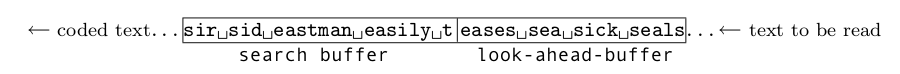
\includegraphics[width=0.8\textwidth]{images/sliding_window_lz77.png}
  \caption{Codificação LZ77 - janela deslizante \citep{salomon2007}.}
  \label{fig:sliding_window_lz77}
  \end{figure}

  \framebreak

  \begin{figure}[h!]
  \centering
  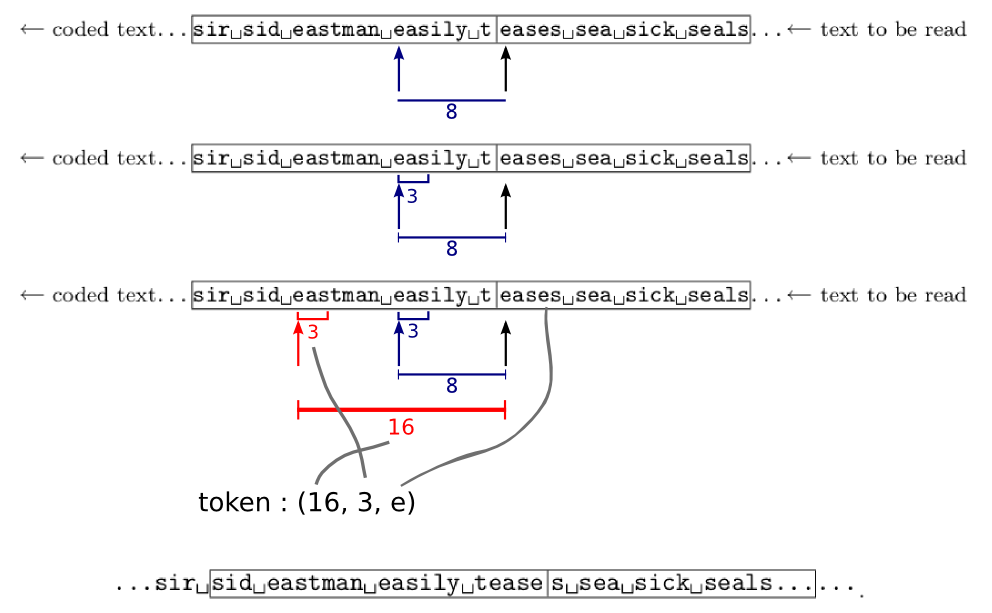
\includegraphics[width=0.65\textwidth]{images/lz77_schema.png}
  \caption{Codificação LZ77 \citep{salomon2007}.}
  \label{fig:lz77_schema}
  \end{figure}

  \framebreak

  O codificador varre o \textit{buffer} de busca (da direita para a esquerda) à procura
  de um \textit{match} para o primeiro símbolo no \textit{look-ahead buffer} (no exemplo em questão o símbolo \textbf{e}).
  O codificador encontra o \textbf{e} da palavra \textbf{easily}. Este \textbf{e} está a uma distância
  de 8 do final do \textit{buffer} de busca. O codificador busca a maior sequência igual (\textit{match}), no
  caso em tela, encontra a sequência \textbf{eas} de comprimento 3. O codificador continua a busca 
  no símbolos passados. No exemplo dado, o codificador encontra outra correspondência (\textit{match}) 
  a uma distância de 16 e, mais uma vez, a maior sequência igual será também de comprimento 3.
  O codificador seleciona a sequência igual mais longa ou, em caso de empate, a última encontrada (para simplificar o codificador).
  Como houve empate no exemplo será gerado o \textit{token} (16, 3, e) constituído por:
  deslocamento (\textit{offset}), comprimento (\textit{length}) e próximo símbolo (\textit{next symbol}) no
  \textit{buffer} de busca.
  As janelas são então deslocadas para a direita $n+1$ posições, onde $n$ é comprimento do último \textit{match} encontrado.
  No nosso exemplo, $n=3$.

  \framebreak

  Se, por um lado, utilizar o último \textit{match} simplifica o codificador, por não ter de manter registro de 
  todos os \textit{matches} encontrados, por outro lado, gera valores de \textit{offset} grandes na saída.
  Isto não parece ser vantajoso. Se selecionarmos o primeiro \textit{match}, teremos valores de \textit{offset}
  pequenos na saída. É possível então seguir a compressão LZ77 por uma codificação Huffman, onde os \textit{offset} menores
  serão codificados por palavras menores. Este método foi proposto por Bernd Herd, sendo conhecido como LZH.

  \framebreak

  Os primeiros 5 passos na codificação do exemplo são apresentadas a seguir:
  \begin{figure}[h!]
  \centering
  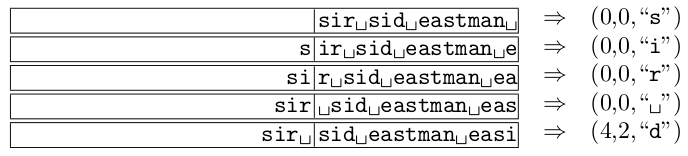
\includegraphics[width=0.7\textwidth]{images/lz77_5steps.png}
  \caption{Passos do LZ77 \citep{salomon2007}.}
  \label{fig:lz77_5steps}
  \end{figure}

  \framebreak

  \textbf{token}: (\textit{offset, length, symbol})
  
  O tamanho do \textit{token} é: tamanho do \textit{offset} + tamanho do comprimento + tamanho do símbolo.
  
  \begin{itemize}
  \item tamanho do \textit{offset} = $\lceil log_2 S \rceil$, onde $S$ é o comprimento do \textit{buffer} de busca (tipicamente de 10 a 12 bits)
  \item tamanho do comprimento = $\lceil log_2 (L-1) \rceil$, onde $L$ é o tamanho do \textit{buffer} de \textit{look-ahead} (tipicamente 5 bits)
  \item tamanho do símbolo = $\lceil log_2 A \rceil$, onde $A$ é o tamanho do alfabeto (tipicamente 8 bits)
  \end{itemize}

  Tamanho total do \textit{token} típico é 11 + 5 + 8 = 24 bits.

  \framebreak 

  \begin{figure}[h!]
  \centering
  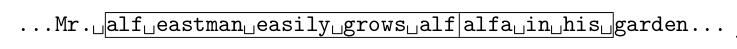
\includegraphics[width=0.7\textwidth]{images/lz77_token_ex01.png}
  %\caption{.}
  \label{fig:lz77_token_ex01}
  \end{figure}
  cria o \textit{token} (3,4,``\underline{\ }'').

  \vspace{2ex}
  \begin{figure}[h!]
  \centering
  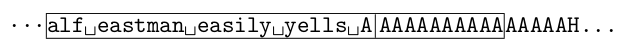
\includegraphics[width=0.7\textwidth]{images/lz77_token_ex02.png}
  %\caption{.}
  \label{fig:lz77_token_ex02}
  \end{figure}
  cria o \textit{token} (1,9,A).

  \framebreak

  O decodificador é bem mais simples.
  Precisa manter um \textit{buffer}, com mesmo tamanho que a janela do codificador:
  \begin{enumerate}
  \item decodificador recebe um \textit{token};
  \item encontra uma correspondência no seu \textit{buffer};
  \item escreve na saída a correspondência encontrada e terceiro campo do \textit{token};
  \item desloca a \textit{string} encontrada e o terceiro campo para dentro do \textit{buffer}.
  \end{enumerate}

  \begin{itemize}
  \item o método assume implicitamente que padrões ocorrem próximos.
  \item O método básico do LZ77 foi melhorado em diversas maneiras aos logo dos anos 80 e 90:
        \begin{itemize}
        \item utilização de campos de \textit{offset} e comprimento com tamanhos variáveis no \textit{token};
        \item aumentar o comprimento de ambos \textit{buffers};
        \item mover todo o texto na janela para a esquerda após cada correspondência encontrada;
        \item substituir a janela linear por uma janela circular;
        \item adicionar um bit extra (\textit{flag}) a cada \textit{token}, eliminando o terceiro campo;
        \item busca com \textit{Deflate algorithm} utilizando \textit{hash table} para encontrar correspondências.
        \end{itemize}
  \end{itemize}

\end{frame}  


\subsection{LZ78}
\begin{frame}[allowframebreaks] 
  \frametitle{LZ78}

  \bibentry{ziv1978}

  \vspace{1ex}
  LZ78 é também conhecido como LZ2.

  O LZ78 não utiliza \textit{buffer} de busca, nem \textit{look-ahead buffer}, ou janela deslizante,
  ao invés, utiliza um dicionário com as strings encontradas previamente.

  \begin{itemize}
  \item dicionário começa vazio (ou quase vazio);
  \item o tamanho do dicionário é limitado pela quantidade de memória disponível;
  \item o codificador escreve na saída \textit{tokens} com dois campos (ponteiro para o dicionário e um símbolo);
  \item cada \textit{token} corresponde a uma \textit{string} de símbolos na entrada;
  \item esta \textit{string} é adicionada ao dicionário após o \textit{token} ser escrito no fluxo de dados comprimido;
  \item nada é apagado do dicionário (dicionário tende a crescer rapidamente e ocupar toda memória).
  \end{itemize}

  \framebreak

  Funcionamento do LZ78:
  \begin{itemize}
  \item O dicionário começa com uma \textit{string} vazia (\texttt{null}) na posição zero.
  \item À medida que os símbolos são codificados, strings são adicionadas no dicionário,
  \item O próximo símbolo \textbf{x} é lido no fluxo de dados de entrada.
  \item Procura-se por \textbf{x} no dicionário.
  \item Se não for encontrado, adiciona-o ao dicionário e gera o seguinte \textit{token} na saída: \textbf{(0, x)}
  \item Se for encontrado, o próximo símbolo \textbf{y} é lido e procura-se no dicionário pela \textit{string} de
        dois símbolos \textbf{xy}.
  \item Se não for encontrado, a \textit{string} \textbf{xy} é adicionada à próxima posição disponível no dicionário e o 
        \textit{token} \textbf{(37, y)} é escrito na saída, onde \textbf{37} é a posição no dicionário onde encontrou-se
        a \textit{string} \textbf{x} (por exemplo).
  \end{itemize}  


  \framebreak
  Estrutura em árvore.
  \begin{itemize}
  \item Uma boa estrutura de dados para o dicionário é uma árvore.
  \item A árvore começa com a \textit{string} vazia na raiz.
  \item Todas strings que começam com a \textit{string} vazia (strings para as quais o ponteiro de \textit{token} é zero) são adicionadas
        como filhos da raiz.
  \item Considerando um alfabeto de símbolos de 8-bits, existem 256 símbolos diferentes, então em princípio, cada nó
        da árvore pode ter até 256 filhos.
  \end{itemize} 

  \framebreak

  \begin{figure}[h!]
  \centering
  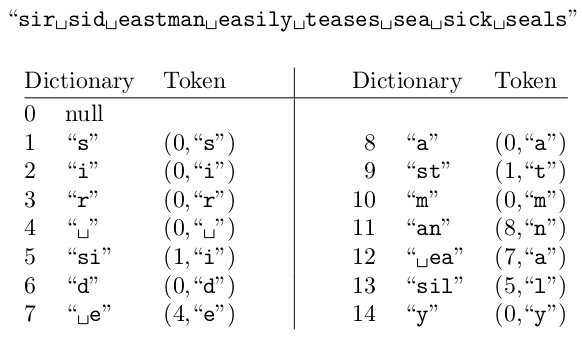
\includegraphics[width=0.7\textwidth]{images/lz78_example.png}
  \caption{Exemplo \citep{salomon2007}.}
  \label{fig:lz78_example}
  \end{figure}
 
  \framebreak

  \begin{figure}[h!]
  \centering
  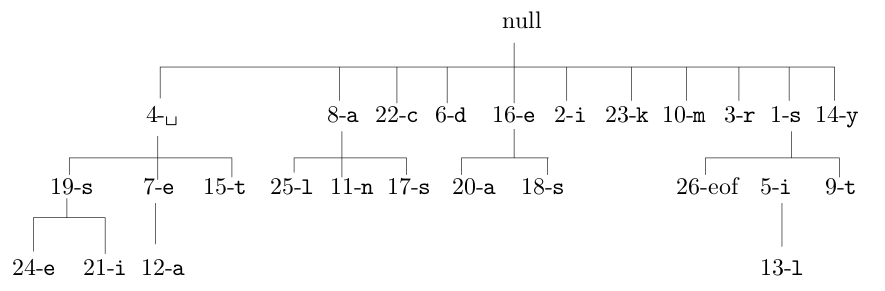
\includegraphics[width=0.8\textwidth]{images/lz78_tree_example.png}
  \caption{Exemplo \citep{salomon2007}.}
  \label{fig:lz78_tree_example}
  \end{figure}

 
\end{frame}

\subsection{LZW}
\begin{frame}[allowframebreaks]
  \frametitle{LZW}
  
  \bibentry{welch1984} 
  \vspace{2ex} 

  LZW é uma variação popular do LZ78, desenvolvida por Terry Welch em 1984. 
  
  \vspace{2ex}
  A sua principal característica é eliminar o segundo campo do \textit{token}.
  (um \textit{token} do LZW consiste em apenas um ponteiro para o dicionário)

  \vspace{2ex}
  O método LZW começa inicializando o dicionário com todos os símbolos do alfabeto.
  Símbolos de 8 bits: 256 entradas.

  \framebreak

  O princípio do LZW é que o codificador recebe os símbolos um a um e acumula-os formando uma \textit{string} \textbf{I}.
  \begin{itemize}
  \item Após cada símbolo ser recebido na entrada e concatenado formando \textbf{I},
        busca-se no dicionário pela \textit{string} \textbf{I}.
  \item Enquanto \textbf{I} for encontrado no dicionário, o processo continua.
  \item Em certo momento, ao adicionar o próximo símbolo \textbf{x} a busca falhará, ou seja,
        a \textit{string} \textbf{I} está no dicionário, mas a \textit{string} \textbf{Ix} não está.
  \item o codificador 
    \begin{itemize}
    \item escreve na saída o ponteiro a localização da \textit{string} \textbf{I} no dicionário 
    \item acrescenta a \textit{string} \textbf{Ix} na próxima posição livre do dicionário
    \item inicializa a \textit{string} de busca \textbf{I} como sendo o símbolo \textbf{x}. 
    \end{itemize}
  \end{itemize}  

  \framebreak

  \begin{figure}[h!]
  \centering
  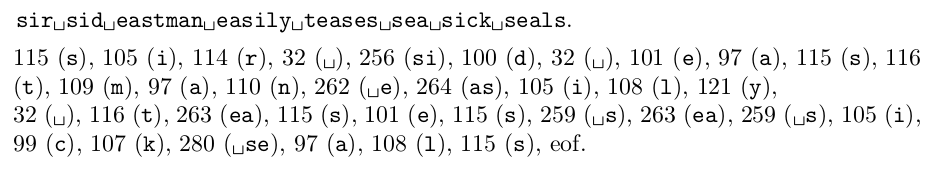
\includegraphics[width=0.8\textwidth]{images/lzw_example.png}
  \caption{Exemplo \citep{salomon2007}.}
  \label{fig:lzw_example}
  \end{figure}

  \framebreak

  \begin{enumerate}
  \item Inicializa o dicionário: as posições 0 a 255 conterão todos os 256 bytes possíveis.
  \item A primeira entrada é o símbolo \textbf{s}. Este é encontrado no dicionário (na posição 115, já que 
        é o valor do código ASCII para \textbf{s}). O próximo símbolo na entrada é \textbf{i}, mas
        \textbf{si} não está no dicionário. O codificado fará o seguinte: (1) a saída será 115,
        (2) salva a \textit{string} \textbf{si} na próxima posição disponível no dicionário (256),
        e (3) inicializa a \textit{string} de busca \textbf{I} com o símbolo \textbf{i}.
   \item O próximo símbolo na entrada do codificador é \textbf{r}, porém a \textit{string} \textbf{ir} 
        não está no dicionário. O codificador (1) emite na saída 105 (código ASCII para \textbf{i}),
        (2) salva \textbf{ir} na próxima posição disponível no dicionário (257), e (3) inicializa
        \textbf{I} com o símbolo \textbf{r}.
   \end{enumerate}

   \framebreak

   \begin{columns}[T]
   \column{.33\textwidth}
   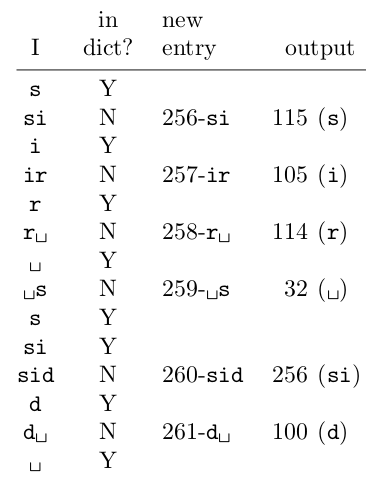
\includegraphics[width=0.9\textwidth]{images/lzw_encoding01.png}
   \column{.33\textwidth}
   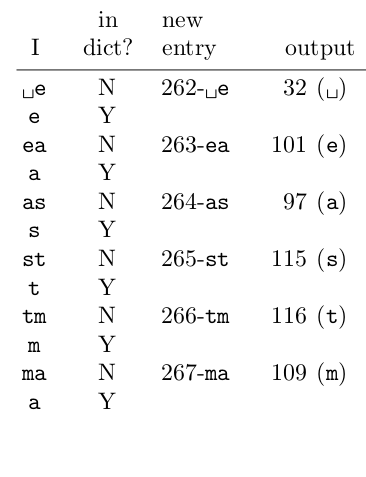
\includegraphics[width=0.9\textwidth]{images/lzw_encoding02.png}
   \column{.33\textwidth}
   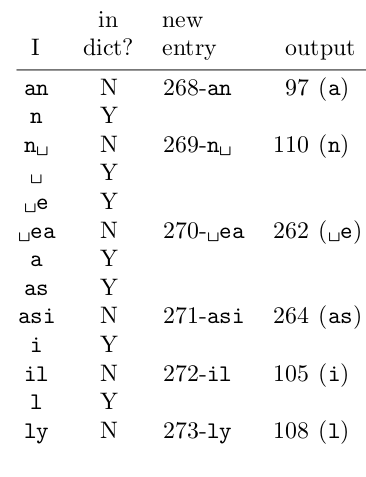
\includegraphics[width=0.9\textwidth]{images/lzw_encoding03.png}
   \end{columns}
   \citep{salomon2007}

   \framebreak

  \begin{figure}[h!]
  \centering
  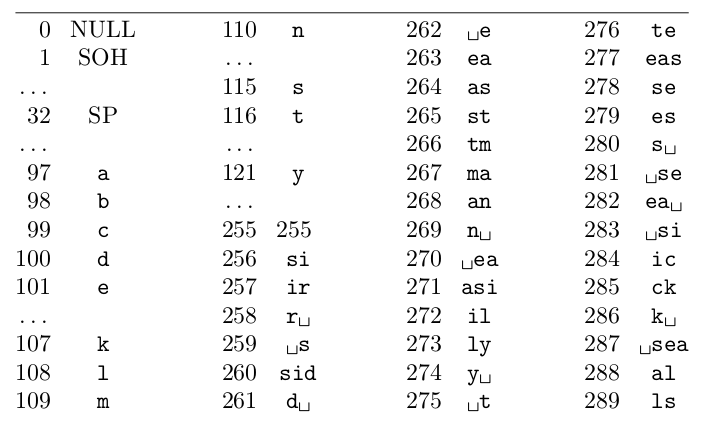
\includegraphics[width=0.65\textwidth]{images/lzw_dictionary.png}
  \caption{Dicionário final. Exemplo \citep{salomon2007}.}
  \label{fig:lzw_dictionary}
  \end{figure}

\end{frame}


\subsection{Análise da compressão Lempel Ziv}
\begin{frame}[allowframebreaks]
  \frametitle{Compressão Lempel Ziv}

  \begin{itemize}
  \item A sequência produzida pela fonte é analisada (\textit{parsed})
	nas menores frases que ainda não ocorreram até então (histórico).
  \item exemplo: a frase `a\textvisiblespace casa\textvisiblespace caiu'
	terá a seguinte análise: \\
	a, \textvisiblespace, c, as, a\textvisiblespace, ca, i, u
  \item exemplo binário: a \textit{string} `1011010100010 ...' será analisada com\\
	1, 0, 11, 01, 010, 00, 10, ...

  \item Para codificar, fornecemos o local do prefixo (\textit{string} que já
	ocorreu antes, exceto o símbolo final) e então adiciona o índice do
	símbolo final. Utiliza-se $0$ como ponteiro nulo, indicando que a \textit{string}
	não ocorreu antes.

  \item exemplo: `a\textvisiblespace casa\textvisiblespace caiu' \\
	\begin{tabular}{lcccccccc}
	frase   & a 	& \textvisiblespace 	& c 	& as 	& a\textvisiblespace 	& ca 	& i 	& u \\
	posição & 1 	& 2			& 3 	& 4 	& 5 			& 6 	& 7 	& 8 \\
	token   & (0,a) & (0,\textvisiblespace) & (0,c) & (1,s) & (1,\textvisiblespace)	& (3,a) & (0,i) & (0,u) 
	\end{tabular}

  \item exemplo binário: `1011010100010 ...' \\
	\begin{tabular}{lcccccccc}
        frase   & 1	& 0	& 11	& 01	& 010	& 00	& 10	\\ 
	posição & 1 	& 2 	& 3 	& 4	& 5	& 6 	& 7	\\
	token   & (0,1) & (0,0) & (1,1) & (2,1) & (4,0) & (2,0) & (1,0) 
	\end{tabular}

  \item De forma geral, à medida que a codificação se procede, os ponteiros referenciam
	\textit{strings} cada vez mais longas, fazendo assim com que a taxa de compressão melhore
	(assumindo que existe regularidade na fonte, gerando \textit{strings} repetidas).
  \end{itemize}

\end{frame}

\begin{frame}[allowframebreaks]
  \frametitle{Lempel Ziv - Codificação Binária}

  Vamos analisar a codificação binária.
  \begin{itemize}
  \item O número de bits necessários para a codificação dependerá do número de frases encontradas
	na \textit{string} gerada pela fonte.
  \item $c(n)$ é o número de frases de uma \textit{string} de comprimento $n$ quando analisada
	seguindo o algoritmo descrito anteriormente.
  \item Serão necessários $\lceil \log c(n) \rceil + 1$ bits, onde o último bit ($+1$) é adicionado 
	para descrever o bit final.
  \item Para o exemplo dado anteriormente (`1011010100010'), teremos $c(n)=7$, e assim:
	{ \scriptsize
        \begin{tabular}{lcccccccc} 
        frase   & 1       & 0       & 11      & 01      & 010     & 00      & 10    \\
        posição & 1       & 2       & 3       & 4       & 5       & 6       & 7     \\
        token   & (0,1)   & (0,0)   & (1,1)   & (2,1)   & (4,0)   & (2,0)   & (1,0) \\
	código  & (000,1) & (000,0) & (001,1) & (010,1) & (100,0) & (010,0) & (001,0 ) 
        \end{tabular}
	}
  \item O processo de decodificação é simples: basta criar uma lista das \textit{strings}
	que já foram encontradas e, quando encontrar $(i,j)$, escreva na saída a \textit{string}
	armazenada na posição $i$ e em seguida escreva $j$.
  \item Quando este procedimento funcionará bem e quando irá falhar para fontes com baixa entropia?
	Teremos uma boa compressão quando houver muita repetição de \textit{strings} e \textit{sub-strings} (ex. texto).
	O processo será ineficiente quando existir correlações esparsas ou que dependam de um extensão muito grande do sinal
	ou quando existir quasi-repetição (ex. sinais amostrados de áudio, imagem, etc).
  \end{itemize}
\end{frame}
\note{
(merriam-webster)

Definition of \textbf{parse}: 

\textit{transitive verb}

\begin{enumerate}
\item to divide (a sentence) into grammatical parts and identify the parts and their relations to each other
\item to examine in a minute way :analyze critically
\end{enumerate}

\textit{intransitive verb}

\begin{enumerate}
\item to give a grammatical description of a word or a group of words
\item to admit of being parsed
\end{enumerate}

}


\begin{frame}[allowframebreaks]
  \frametitle{Lempel Ziv}
  \begin{itemize}
  \item Vamos considerar um alfabeto binário $\mathcal{X} = \{0,1\}$.
  \end{itemize}

  \begin{definition}[Análise (\textit{parsing})]
  Uma análise (\textit{parsing}) $S$ de uma \textit{string} $x_1,x_2, \ldots, x_n$ é
  uma divisão da \textit{string} em frases, separadas por vírgulas (ou outro separador qualquer).
  \end{definition}

  \begin{definition}[Análise Distinta (\textit{distinct parsing})]
  Uma análise distinta (\textit{distinct parsing}) é uma análise (\textit{parsing})
  em que não existe duas frases idênticas.
  \end{definition}

  \begin{itemize}
  \item Ex. 01101101. Uma análise possível é: 0,11,0,11,01. Mas esta não é distinta.
  \item Uma análise distinta de 01101101 seria 0,1,10,11,01.
  \item Lempel-Ziv produz uma análise distinta da sequência da fonte.

  \item Seja $c(n)$ o número de frases na análise LZ de uma \textit{string} de comprimento $n$.
	Então $c(n)$ depende da \textit{string} $x_{1:n}$. ($c=c(n)=c(x_{1:n})$)
  \item Após a compressão, teremos uma sequência de $c(n)$ pares da forma (ponteiro, bit),
	onde o ponteiro requer $\lceil \log c(n) \rceil$ bits.
  \item O comprimento da sequência comprimida será
	\begin{equation}
	c(n) ( \lceil \log c(n) \rceil + 1 ) \text{ bits}
	\end{equation}
  \item Queremos que a compressão LZ atinja o limite da taxa de entropia, ou seja,
	queremos
	\begin{equation}
	\frac{c(n) ( \lceil \log c(n) \rceil + 1 )}{n} \rightarrow H(X)
	\end{equation}
	para uma sequência estacionária ergódica $x_{1:n}$, ou seja,
	\begin{equation}
	\frac{1}{n} \E_{p(x_{1:n})} \left[ c(X_{1:n}) (\lceil \log c(X_{1:n}) \rceil + 1) \right]  = H(X)
	\end{equation}
  \end{itemize}

\end{frame}


\begin{frame}[allowframebreaks]
  \frametitle{Dominância}
  \begin{itemize}
  \item Dominância (\textit{little-o notation})
	\begin{equation}
	o(g(n)) \triangleq \{ f(n) : \forall c > 0, \exists n_0 > 0 \quad / \quad 0 \leq f(n) \leq c g(n), \forall n \geq n_0 \}
	\end{equation}
	ou seja, $o(g(n))$ é o conjunto de todas as funções dominadas por $g$.
  \item Intuitivamente, isto significa que $g(n)$ cresce muito mais rápido do que uma função
	$f(n) \in o(g(n))$ qualquer (o crescimento de $f(n)$ não é nada comparado ao de $g(n)$).
  \item Se $g(n)$ não é nulo, então para qualquer $f \in o(g(n))$, teremos $\lim_{n \rightarrow \infty} f(n)/g(n) = 0$.
  \item As funções $o(1)$ são funções que tendem a zero no limite, isto é
	\begin{equation}
	o(1) \triangleq \{ f(n) : \forall c > 0 , \exists n_0 > 0 \quad / \quad 0 \leq f(n) < c, \forall n \geq n_0 \}
	\end{equation}
	isto é, se $f \in o(1)$, então $\lim_{n \rightarrow \infty} f(n) = 0$.
  \end{itemize}
\end{frame}

\begin{frame}[allowframebreaks]
  \frametitle{Lempel-Ziv: Demonstração}

  \begin{lemma}[limite superior do número de frases]
  O número de frases $c(n)$ em qualquer análise (\textit{parsing}) distinta de sequências
  binárias $x_{1:n}$ satisfaz:
	\begin{equation}
	c(n) \leq \frac{n}{(1-\epsilon_n) \log n}
	\end{equation}
  onde $\epsilon \rightarrow 0$ e $n \rightarrow \infty$. Ou seja,
	\begin{equation}
	c(n) \leq \frac{n}{\log n} (1 + o(1))
	\end{equation}

  nota: 
	\begin{equation}
	\frac{1}{1 - \epsilon} = \underbrace{ \frac{1}{1 - \epsilon} - 1 }_{\in o(1)} + 1
	\end{equation}
  \end{lemma}

  \begin{proof}
	\begin{itemize}
	\item Na demonstração utilizaremos a seguinte igualdade:
		\begin{equation}
		\sum_{l=1}^k 2^l = \sum_{l=0}^k 2^l - 1 = 2^{k+1} - 2
		\end{equation}
	\item Seja $n_k$ a soma de todos os comprimentos de todas as \textit{strings} distintas
		de comprimento $\leq k$ (a soma do comprimento de todas as \textit{strings} no
		dicionário, ou o tamanho do dicionário). 
		Para um dado comprimento $j$, existem $2^j$ \textit{strings} binárias distintas.

		\begin{equation}
		n_k = \sum_{j=1}^k j 2^j
		\end{equation}

	\end{itemize}
	\proofbreak

	Na demonstração abaixo iremos utilizar que $\sum_{l=1}^k 2^l = 2^{k+1} - 2$.
	\begin{eqnarray}
	n_k &=& \sum_{j=1}^k j 2^j = \sum_{j=1}^k 2^j + \sum_{j=2}^k 2^j + \ldots + \sum_{j=k}^k 2^j = \sum_{l=1}^k \sum_{j=l}^k 2^j \nonumber \\
	&=& \sum_{l=1}^k \left( \sum_{j=1}^k 2^j  - \sum_{j=1}^{l-1} 2^j \right) = \sum_{l=1}^k \left( 2^{k+1} - 2 - ( 2^{l} - 2 ) \right) \nonumber \\
	&=& k 2^{k+1} - \sum_{l=1}^k 2^{l} = k 2^{k+1} - (2^{k+1} - 2) = (k-1) 2^{k+1} + 2 
	\end{eqnarray}

	\proofbreak
	Considere uma \textit{string} binária de comprimento $n$. Observe que o número de frases
	distintas $c(n)$ desta \textit{string} será maximizado quando todas as frases forem tão menores quanto possível.

	\begin{itemize}
	\item Vamos inicialmente considerar o caso em que $n = n_k$ (ou seja, vamos considerar uma
	\textit{string} de comprimento $n$ igual à soma dos comprimentos de todas as \textit{strings}
	distintas de comprimento $\leq k$). Então $c$ será maximizado quando considerarmos todas
	as \textit{strings} distintas de comprimento $\leq k$. Iremos considerar $k \geq 2$,
	para que tenhamos efetivamente \textit{strings}.
	\end{itemize}

	\proofbreak
	O número de \textit{strings} distintas de comprimento $\leq k$ é
	\begin{equation}
	c(n) = c(n_k) \leq \sum_{j=1}^k 2^j = 2^{k+1} - 2 < 2^{k+1} < \frac{n_k}{k-1} = \frac{n}{k-1} ,
	\end{equation}
	onde utilizamos $\sum_{j=1}^k 2^j = 2^{k+1} - 2$, como visto anteriormente, e $\frac{n_k}{k-1} > 2^{k+1}$,
	pois

	\proofbreak

	\begin{eqnarray}
	n_k &=& (k-1) 2^{k+1} + 2 \nonumber \\
	n_k - 2 &=& (k-1) 2^{k+1} \nonumber \\
	n_k &>& (k-1) 2^{k+1} \nonumber \\
	\frac{n_k}{k-1} &>& 2^{k+1} 
	\end{eqnarray}

	\proofbreak

	\begin{itemize}
        \item Vamos agora considerar o caso em que $n \neq n_k$.
	\end{itemize}

	Note que:
	\begin{equation}
	n_k + (k+1) 2^{k+1} = 2k 2^{k+1} + 2 = k 2^{k+2} + 2 = n_{k+1}
	\end{equation}
	onde novamente utilizamos $n_k = (k-1) 2^{k+1} + 2$.

	\proofbreak
	\begin{itemize}
        \item Supondo $n_k \leq n < n_{k+1}$, digamos que $n = n_k + \delta_k$ com
		$\delta_k < (k+1)2^{k+1} = n_{k+1} - n_k$ (que é o próximo passo de $n_k$).

	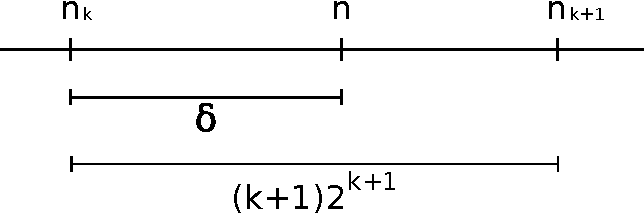
\includegraphics[width=0.6\linewidth]{images/nnkinterval.pdf}
	\end{itemize}

	\proofbreak
	\begin{itemize}
        \item Considerando \textit{strings} de comprimento $n_k \leq n < n_{k+1}$,
		ao realizar a análise (\textit{parsing}) em frases distintas 
		com menor comprimento possível, teremos $c(n)$ maximizado quando:
		\begin{enumerate}
		\item não utilizarmos frases com comprimento maior que $k+1$;
		\item e utilizarmos todas as frases com comprimento $\leq k$, sendo
			que existem $c(n_k) < n / (k-1)$;
		\item as \textit{strings} remanescentes, $(n - n_k) = \delta$, serão 
			analisadas em frases únicas de comprimento $k+1$, então existe
			um total de $\delta / (k+1)$ dessas \textit{strings}.
		\end{enumerate}
	\end{itemize}
	\proofbreak

	Teremos então:
	\begin{equation}
	c(n) < \frac{n_k}{k-1} + \frac{\delta}{k+1} < \frac{n_k + \delta}{k - 1} = \frac{n}{k - 1} ,
	\end{equation}
	onde $k$ é tal que $n_k \leq n < n_{k+1}$.

	\proofbreak

	\begin{itemize}
	\item para um dado $n$, vamos considerar $n_k \leq n < n_{k+1}$;
	\item vamos limitar $k$ dado $n$ (onde $n$ é o comprimento da \textit{string} e
		$k$ é o comprimento da maior frase de análise);
	\item como $n \geq n_k = (k-1)2^{k+1} + 2 > 2^k$, teremos $k < \log n$
		\begin{eqnarray}
		n &\geq& n_k = (k-1)2^{k+1} + 2 \nonumber \\
			&=& \underbrace{(k-1)}_{\geq 1} 2 \times 2^k + 2 > 2^k .
	%		&=& k 2^{k+1} - 2 \underbrace{ (2^k - 1) }_{\geq 1 \atop \text{já que } k \geq 1 } \\
	%		&>& k 2^{k+1} > 2^{k+1} > 2^k
		\end{eqnarray}
	onde utilizamos que $k \geq 2$, como argumentado anteriormente.
	\end{itemize}

	\proofbreak

        \begin{itemize}
	\item teremos também
		\begin{eqnarray}
		n &<& n_{k+1} = k 2^{k+2} + 2 < (k+2) 2^{k+2} \nonumber \\
			&<& (\log n + 2) 2^{k+2} 
		\end{eqnarray}
		onde utilizamos que $k < \log n$.
	\item teremos assim
		\begin{equation}
		k+2 > \log \left( \frac{n}{\log n + 2} \right)
		\label{eq-kp2}
		\end{equation}
	\end{itemize}

	\proofbreak

        \begin{itemize}
        \item Para $n \geq 4$, iremos subtrair 3 de cada lado da Equação \ref{eq-kp2}:
	\vspace{-1em}
	\begin{eqnarray}
	k - 1 &>& \log n - \log( \log n + 2 ) - 3 \nonumber \\
		&=& \left( 1 - \frac{\log( \log n + 2 ) + 3}{\log n} \right) \log n \nonumber \\
		&\geq& \left( 1 - \frac{\log( 2 \log n ) + 3}{\log n} \right) \log n \quad {\small \text{, utilizando \ } n \geq 4 \Rightarrow \log n \geq 2} \nonumber \\
		&=& \left( 1 - \frac{\log( \log n ) + 4}{\log n} \right) \log n = \left( 1 - \epsilon_n \right) \log n 
	\end{eqnarray}
	onde
	\vspace{-1em} 
	\begin{equation}
	\epsilon_n = \min \left\{ 1, \frac{\log \log n + 4}{\log n} \right\} \rightarrow 0 .
	\end{equation}
        \end{itemize}

	\proofbreak

        \begin{itemize}
        \item Utilizando que $k-1 \geq 0$ e também
		\begin{equation}
		c(n) \leq \frac{n}{k-1} ,
		\end{equation}
		como visto anteriormente, teremos 
		\begin{equation}
                c(n) \leq \frac{n}{k-1} \leq \frac{n}{(1 - \epsilon_n)\log n} = \frac{n}{\log n} \left( 1 + o(1) \right) .
		\end{equation}
	\end{itemize}
  %\proofbreak
  \end{proof}
\end{frame}
\note{

\begin{eqnarray}
\sum_{l=0}^{k} 2^l &=& 1 + 2 + 4 + \ldots + 2^k \nonumber \\
(1 - 2) \left( \sum_{l=0}^{k} 2^l \right) &=& ( 1 + 2 + 4 + \ldots + 2^k ) (1 - 2) \nonumber \\
(-1) \sum_{l=0}^{k} 2^l &=& 1 - 2^{k+1} \nonumber \\
\sum_{l=0}^{k} 2^l &=&  2^{k+1} - 1 
\end{eqnarray}
}


\begin{frame}[allowframebreaks]
  \frametitle{Distribuição de Máxima Entropia}

  \begin{theorem}[Distribuição de Máxima Entropia]
  Seja $f$ uma função densidade probabilidade com suporte $S$ (ou seja,
  $\int_S f(x) dx = 1$) satisfazendo as seguintes restrições de momento
	\begin{equation}
	\int_S f(x) r_i(x) dx = \alpha_i \quad , 1 \leq i \leq m .
	\end{equation}
  A função de densidade da forma $f_{\lambda}(x) = e^{\lambda_0 + \sum_{i=1}^{m} \lambda_i r_i (x)}$,
  onde $\lambda = (\lambda_0, \ldots, \lambda_m)$ é escolhido de forma que $f_{\lambda}(x)$ satisfaça 
  as restrições, é a única distribuição que satisfaz as restrições e maximiza a 
  entropia diferencial $h(f)$.
  \end{theorem}

  \begin{itemize}
  \item Demonstração: capítulo 12 (utiliza multiplicadores de Lagrange).
  \item A distribuição Gaussiana, para um dada média ($\E X = \mu$) e covariância ($\E X X^T = C$), 
	é a única distribuição com entropia máxima.
  \end{itemize}

  \framebreak

  \begin{lemma}[limite da entropia]
  Seja $Z$ uma v.a. inteira positiva com média $\mu$. Podemos limitar $H(Z)$ da seguinte forma:
	\vspace{-1em}
	\begin{equation}
	H(Z) \leq (\mu + 1) \log (\mu + 1) - \mu \log \mu .
	\end{equation}
  \end{lemma}
   %
  \begin{proof}[ideias para a demonstração]
  \begin{itemize}
  \item Uma v.a. $Z$ com distribuição geométrica (definida nos inteiros $1,2,\ldots$)
	com média $\mu = 1/p$ é definida como $\Pr(Z=k) = (1-p)^k p$.
  \item A entropia da distribuição geométrica com média $\mu$ é dada por
	$(\mu+1) \log(\mu +1) - \mu \log \mu$.
  \item A distribuição geométrica é a distribuição com máxima entropia dentre todas aquelas
	definidas nos inteiros positivos com média $\mu$ (mais uma vez utilizando 
	os multiplicadores de Lagrande para demonstrar).
  \end{itemize}
  \end{proof}
\end{frame}


\begin{frame}[allowframebreaks]
  \frametitle{Ergodicidade}
  \begin{itemize}
  \item Processos ergódicos não podem ser separados em diferentes modos comportamentais persistentes.
  \item A média temporal é a mesma que a média amostral.
  \item Seja $x = \{x_i\}$ uma sequência de letras produzida pela fonte.
  \item $T^l x$ é a sequência deslocada no tempo de $l$ posições. 
	Se $T^l x = x'$, então $x'_i = x_{i+l}$, $\forall i$.
  \item Chamaremos de $S$ um conjunto infinito de sequências de símbolos da fonte,
	isto é, $S = \{x : x \text{ é uma sequência de símbolos da fonte } \}$.
  \item $T^l S$ é o conjunto de todas as sequências deslocadas de $l$ posições, isto é,
	se $x' = T^l x$, então $x' \in T^l S$ se $x \in S$.
  \item Um conjunto $S$ é \textbf{invariante} se $T^l S = S$, $\forall l$.
	\begin{itemize}
	\item exemplo: o conjunto de todas as sequências de uma fonte com alfabeto discreto é invariante.
	\item exemplo: $S = \{ \ldots 000 \ldots , \ldots 111 \ldots \}$ é invariante.
	\item exemplo: para qualquer sequência $x$, o conjunto
		\begin{equation}
		\{ \ldots, T^{-2}x, T^{-1}x, T^{0}x, T^1 x, T^2 x , \ldots  \}
		\end{equation}
		é invariante (o conjunto de todas os possíveis deslocamentos de uma sequência $x$).
	\end{itemize}
  \item Uma fonte estacionária discreta é \textbf{ergódica} se todo conjunto invariante de
	sequências possuir probabilidade $1$ ou $0$, ou seja,
		\begin{equation}
		\Pr \{ S: T^l S = S, \forall l \} = 1 \text{ ou } 0, \quad \forall S .
		\end{equation}
  \end{itemize}
\end{frame}


\begin{frame}[allowframebreaks]
  \frametitle{Aproximação de Markov de ordem $k$}
  \begin{itemize}
  \item Seja $\{X_i\}_{i=-\infty}^{\infty}$ um processo estacionário ergódico com função
	massa de probabilidade $p(x_1, x_2, \ldots, x_n)$, então para um inteiro $k$ fixo,
	definimos a aproximação de ordem $k$ para $p$ como
	\begin{equation}
	Q_k( \underbrace{ x_{-(k-1)}, \ldots, x_0}_{\text{estado passado}}, x_1, \ldots, x_n  ) \triangleq p(x_{-(k-1):0}) \prod_{j=1}^{n} p(x_j | x_{j-k:j-1})
	\end{equation}
	onde interpretamos $x_{-(k-1):0}$ como o estado `0', $x_{j-k:j-1}$ como o estado `j' e 
	$x_{i:j} \triangleq \{x_i, x_{i+1}, \ldots, x_j \}$ com $i \leq j$.
  \item Note que $p(x_n | x_{n-k:n-1})$ é estacionário e ergódico, visto que $p(x_{n-k:n})$ também é.
  \item Teremos que
	\begin{eqnarray}
	- \frac{1}{n} \log Q_k(x_1,\ldots,x_n|x_{-(k-1):0}) &=& - \frac{1}{n} \sum_{j=1}^{n} \log p(x_j | x_{j-k:j-1}) \nonumber \\
	\rightarrow - \E \log p(X_j | X_{j-k:j-1}) &=& H(X_j | X_{j-k:j-1}) 
	\end{eqnarray}
	já que o processo é estacionário ergódico.
  \item Iremos mostrar que
	\begin{equation}
	\limsup_{n \rightarrow \infty} \frac{c(n) \log c(n)}{n} \leq H(X_j | X_{j-k : j-1}) \rightarrow H(\mathcal{X})
	\end{equation}
	onde $H(\mathcal{X})$ é a taxa de entropia do processo estocástico.
  \end{itemize}
\end{frame}

\begin{frame}[allowframebreaks]
  \frametitle{Notações}
  \begin{itemize}
  \item Uma \textit{string} $x_{1:n}$, com $x_i \in \mathcal{X}$, será analisada (\textit{parsed}) 
	em $c$ frases distintas, $x_{1:n} = y_1 y_2 \ldots y_c$ onde $y_i$, para $i \in \{1, \ldots, c\}$,
	é uma subsequência.
  \item Faremos $v_i$ o índice em $x_{1:n}$ do início da $i$-ésima frase, ou seja,
	$y_i = x_{v_i:v_{i+1}-1}$ para todo $i=1,2,\ldots,c$.
  \item Os $k$ símbolos de $x_{1:n}$ que antecedem $y_i$ serão chamados de $s_i$, ou seja,
	$s_i = x_{v_i-k : v_i - 1}$. Para $i=1$ teremos $s_1 = x_{-(k-1):0}$, então
	$s_i$ é p `estado' ou o prefixo da $i$-ésima frase.
	
	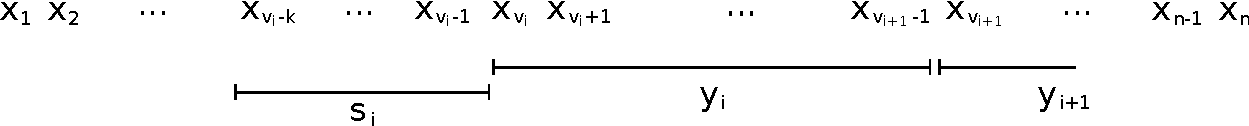
\includegraphics[width=0.9\textwidth]{images/xparse.pdf}
  \item Para $l \in \{1, 2, \ldots, n\}$ e $s \in \mathcal{X}^k$ (uma \textit{string} de comprimento $k$),
	vamos definir $c_{ls}$ como o número de frases em $x_{1:n}$ com comprimento $l$ e que possuem
	como estado anterior $s$, ou seja, $c_{ls}$ é o número de frases de comprimento $l$ precedidas
	por $s$, ou ainda
		\begin{equation}
		c_{ls} = \vert \{ i : i \in \{1, \ldots, c\}, |y_i| = l, s_i = s \} \vert .
		\end{equation}
  \item Teremos assim $\sum_{l,s} c_{ls} = c = c(n)$, onde $c=c(n)$ é o número total de frases
	em uma análise em frases distintas de uma sequência de comprimento $n$.
  \item E ainda, $\sum_{l,s} l c_{ls} = n$, que é o comprimento total da \textit{string}.
  \item Pergunta central: podemos relacionar (ou ao menos limitar) a probabilidade a
	algum aspecto determinístico de uma análise (\textit{parsing})? Veremos como isso é possível,
	e assim poderemos usar a análise baseada no \textit{parsing} para impor um limite sobre a taxa de 
	entropia do processo.
  \end{itemize}

  \begin{lemma}[Desigualdade de Ziv]
  Para qualquer análise (\textit{parsing}) distinta (o que inclui a análise do LZ) de uma \text{string}
  $x_{1:n}$, temos:
	\begin{equation}
	\log Q_k (x_1, \ldots, x_n | s_1) \leq - \sum_{l,s} c_{ls} \log c_{ls}
	\end{equation}
  \end{lemma}

  \begin{itemize}
  \item Note que o limite é independente de $Q$ e depende apenas de $c_{ls}$, que é o 
	número de frases de comprimento $l$ e antecedidas por $s$ (estado anterior).
  \item Ideia principal: quanto maior for a diversidade em $x_{1:n}$, a maior probabilidade
	possível diminui, ou seja, $y_i$'s distintas aumentam a diversidade.
  \end{itemize}


  \begin{proof}[Desigualdade de Ziv]
  \begin{itemize}
  \item Inicialmente temos
	\begin{equation}
	Q_k(x_{1:n}|s_1) = Q_k(y_{1:c} | s_1) = \prod_{i=1}^c p(y_i | s_i)
	\end{equation}
  que segue ao assumir Markovidade de ordem $k$, ou seja, que $y_i$ não depende de
  nada no passado, dado o passado imediato $s_i$.
  \end{itemize}
  \proofbreak
  \begin{itemize}
  \item Temos então, tomando o $\log$ da equação anterior,
	\begin{eqnarray} 
	\log Q_k (x_1, \ldots. x_n | s_1) &=& \sum_{i=1}^{c} \log p(y_i | s) \nonumber \\
		&=& \sum_{l,s} \sum_{i: |y_i| = l, s_i = s} \log p(y_i | s_i) \nonumber \\
		&=& \sum_{l,s} c_{ls} \sum_{i: |y_i| = l, s_i = s} \frac{1}{c_{ls}} \log p(y_i | s_i)
	\end{eqnarray}
  \end{itemize}
  \proofbreak
  \begin{itemize}
  \item entretanto, temos uma mistura cujos coeficientes somam um, pois
	\begin{equation}
	\sum_{i: |y_i| = l, s_i = s} \frac{1}{c_{ls}} = 1
	\end{equation}
	já que $c_{ls}$ é o número de frases de comprimento $l$, antecedidas por $s$,
	e que as somas somam sobre todos os termos. Podemos assim ver esse valores ($1/c_{ls}$)
 	como uma distribuição.
  \end{itemize}
  \proofbreak
  \begin{itemize}
  \item Utilizando a desigualdade de Jensen para o termo em parênteses, teremos
	\begin{equation}
	\sum_{l,s} c_{ls} \left( \sum_{i: |y_i| = l, s_i = s} \frac{1}{c_{ls}} \log p(y_i | s_i) \right) \leq
		\sum_{l,s} c_{ls} \log \left( \sum_{i: |y_i| = l, s_i = s} \frac{1}{c_{ls}} p(y_i | s_i) \right) 
	\end{equation}
  \item Mas todos os $y_i$'s são distintos (não são contabilizados duplamente no somatório), e assim
	\begin{equation}
	\sum_{i: |y_i| = l, s_i = s} p(y_i | s_i) \leq \sum_{y'} p(y'|s) = 1
	\end{equation}
  \end{itemize}
  \proofbreak
  \begin{itemize}
  \item Teremos então o seguinte resultado, para qualquer distribuição,
	\begin{eqnarray}
	\log Q_k (x_1, \ldots. x_n | s_1) &\leq& \sum_{l,s} c_{ls} \log \left( \sum_{i: |y_i| = l, s_i = s} \frac{1}{c_{ls}} p(y_i | s_i) \right) \nonumber \\
		&\leq& \sum_{l,s} c_{ls} \log \left( \frac{1}{c_{ls}} \right) .
	\end{eqnarray}
	Obtivemos um limite que depende exclusivamente da análise (\textit{parsing}).
  \end{itemize}

%  \proofbreak
  \end{proof}
\end{frame}


\begin{frame}[allowframebreaks]
  \frametitle{Teorema Principal}
 
  \begin{theorem}[limite superior é a taxa de entropia]
  Seja $X_{1:n}$ um processo estacionário ergódico com taxa de entropia $H(\mathcal{X})$,
  e $c(n)$ o número de frases em um \textit{parsing} distinto de uma amostra de comprimento $n$
  deste processo. Então
	\begin{equation}
	\limsup_{n \rightarrow \infty} \frac{c(n) \log c(n)}{n} \leq H(\mathcal{X}) 
	\end{equation}
  com probabilidade 1.
  \end{theorem} 
  \note{
	\begin{equation}
	\limsup_{n \rightarrow \infty} a_n \triangleq \inf_{n > 0} \left( \sup_{k > n} a_k \right) = \inf S
	\end{equation}
	onde $S = \{ a: a = \sup_n B_n , \text{ com } B_n=\{a_n, a_{n+1}, \ldots \} \}$.

	\begin{itemize}
	\item exemplo: $\lim_{x \rightarrow \infty} \sin(x)$ não existe, mas 
		$\limsup_{x \rightarrow \infty} \sin(x) = 1$.
	\end{itemize}

	Temos também
	\begin{equation}
	\limsup_{n \rightarrow \infty} a_n \triangleq \sup_{n > 0} \left( \inf_{k>n} a_k \right)
	\end{equation}
	então, $\limsup$ requer a convergência do supremo no máximo local.
  }
\end{frame}



\begin{frame}[allowframebreaks]
  \frametitle{Teorema Principal - demonstração}
  \begin{proof}[limite superior é a taxa de entropia]
  Para simplificar escreveremos $c$ para $c(n)$. 
  \begin{itemize}
  \item Utilizando a desigualdade de Ziv temos
	\begin{eqnarray}
	\log Q_k (x_1,\ldots,x_n | s_1) &\leq& - \sum_{l,s} \frac{c_{ls} c}{c} \log \frac{c_{ls} c}{c} \nonumber \\
		&=& -c\log c - c \sum_{l,s} \frac{c_{ls}}{c} \log \frac{c_{ls}}{c} 
	\end{eqnarray}
  \item como $\sum_{l,s} c_{ls} = c$, vamos escrever $\pi_{ls} = c_{ls}/c$, que pode ser tratado como uma probabilidade,
	já que $\pi_{ls} \geq 0$ e $\sum_{l,s} \pi_{ls} = 1$.
  \end{itemize}
  \proofbreak
  \begin{itemize}
  \item Como $\sum_{l,s} l c_{ls} = n$, temos
	\begin{equation}
	\sum_{l,s} l \pi_{ls} = n/c .
	\end{equation}
  \item Vamos definir duas v.a. U e V, tais que
	\begin{equation}
	p(U=l, V=s) = \pi_{ls}
	\end{equation} 
 	de forma que
	\begin{equation}
	EU = \sum_l l \pi_l = \sum_l l \sum_s \pi_{ls} = n/c 
	\end{equation}
  \end{itemize}
  \proofbreak
  \begin{itemize}
  \item Isto nos leva imediatamente a
	\begin{eqnarray}
	\log Q_k (x_{1:n} | s_1) &\leq& \sum_{ls} c_{ls} \log 1/c_{ls} \nonumber \\
		&=& -c\log c - c \sum_{l,s} \frac{c_{ls}}{c} \log \frac{c_{ls}}{c} \nonumber \\
		&=& c H(U,V) - c\log c .
	\end{eqnarray}
  \end{itemize}
  \proofbreak

  \begin{equation}
  \underbrace{- \frac{1}{n} \log Q_k (x_{1:n} | s_1) }_{\rightarrow \text{ taxa de entropia quando } \atop k \rightarrow \infty \text{ e } n \rightarrow \infty } 
	\geq \underbrace{ \frac{c}{n} \log c }_{\begin{subarray}{c} c=c(n), \\ \text{ queremos mostrar que } \\ \text{converge para entropia de $X$} \end{subarray}} 
	- \underbrace{ \frac{c}{n} H(U,V) }_{\text{idealmente } \rightarrow 0 \atop \text{quando } n \rightarrow \infty} 
  \end{equation}

  \begin{itemize}
  \item Sabemos que $H(U,V) \leq H(U) + H(V)$.
  \item E também $H(V) \leq \log \vert \{0,1\} \vert^k = k$. Podemos pensar em $V$ como uma variável de estado
	(\textit{string} binária de comprimento $k$).
  \end{itemize}
  \proofbreak
  \begin{itemize}
  \item Utilizando o lemma anterior, 
        \begin{equation}
        H(Z) \leq (\mu + 1) \log (\mu + 1) - \mu \log \mu ,
        \end{equation}	
	teremos:
	\begin{equation}
	H(U) \leq (\E U + 1) \log (\E U + 1) - \E U \log \E U
	\end{equation}
  \end{itemize}

  \proofbreak
  \vspace{-1em}
  \begin{eqnarray}
  H(U) &\leq& (\E U + 1) \log (\E U + 1) - \E U \log \E U \nonumber \\
	&=& \left( \frac{n}{c} + 1 \right) \log \left( \frac{n}{c} + 1 \right) - \frac{n}{c} \log \frac{n}{c} \nonumber \\
	&=& \frac{n}{c} \log \left( \frac{n}{c} + 1 \right) + \log \left( \frac{n}{c} + 1 \right) - \frac{n}{c} \log \frac{n}{c} \nonumber \\
	&=& \frac{n}{c} \log \left( \frac{c}{n} \left( \frac{n}{c} + 1 \right) \right) + \log \left( \frac{n}{c} + 1 \right) \nonumber \\
	&=& \frac{n}{c} \log \left( \frac{c}{n} \times \frac{n}{c} + \frac{c}{n} \right) + \log \left( \frac{n}{c} + 1 \right) \nonumber \\
	&=& \frac{n}{c} \log \left( \frac{c}{n} + 1 \right) + \log \left( \frac{n}{c} + 1 \right) + \log \left( \frac{c}{n} + 1 \right) - \log \left( \frac{c}{n} + 1 \right) \nonumber \\
	&=& \left( \frac{n}{c} + 1 \right) \log \left( \frac{c}{n} + 1 \right) + \log \left( \frac{\frac{n}{c} + 1}{\frac{c}{n} + 1} \right) 
  \end{eqnarray}
  \proofbreak
  \begin{eqnarray}
  H(U) &\leq& \ldots \nonumber \\
	&=& \left( \frac{n}{c} + 1 \right) \log \left( \frac{c}{n} + 1 \right) + \log \left( \frac{\frac{n}{c} + 1}{\frac{c}{n} + 1} \right) \nonumber \\
	&=& \left( \frac{n}{c} + 1 \right) \log \left( \frac{c}{n} + 1 \right) + \log \frac{n}{c}
  \end{eqnarray}

  \proofbreak

  Temos então
  \begin{eqnarray}
  \frac{c}{n} H(U,V) &\leq& \frac{c}{n} H(V) + \frac{c}{n} H(U) \nonumber \\
	&\leq& \frac{c}{n} k + \frac{c}{n} \log \frac{n}{c} + \frac{c}{n} \left( \frac{n}{c} + 1 \right) \log \left( \frac{c}{n} + 1 \right) \nonumber \\
	&=& \frac{c}{n} k + \frac{c}{n} \log \frac{n}{c} + \left( \frac{c}{n} + 1 \right) \log \left( \frac{c}{n} + 1 \right) \nonumber \\
	&=& \frac{c}{n} k + \frac{c}{n} \log \frac{n}{c} + 
		\underbrace{ \frac{c}{n} \log \left( \frac{c}{n} + 1 \right) }_{\rightarrow 0 \text{ quando } n \rightarrow \infty} 
		+ \underbrace{ \log \left( \frac{c}{n} + 1 \right) }_{\rightarrow 0 \text{ quando } n \rightarrow \infty} 
  \end{eqnarray}
 
  \proofbreak
   Assim,
  \begin{equation}
  \frac{c}{n} H(U,V) \leq \underbrace{ \frac{c}{n} k }_{\rightarrow 0 \text{ quando } n \rightarrow \infty} + 
		\frac{c}{n} \log \frac{n}{c} + \underbrace{ o(1) }_{\rightarrow 0}
  \end{equation}
  
  Vamos utilizar o lemma (visto anteriormente):
  \begin{equation}
  c(n) \leq \frac{n}{\log n} (1 + o(1)) \leq \frac{n}{c} 
  \end{equation}
  para $n$ grande suficiente e vamos analisar o termo $\frac{c}{n} \log \frac{n}{c}$
  
  \proofbreak
  \begin{itemize}
  \item $1/x \log x$ é monótono até o pico em $x=e$  
  \end{itemize}
  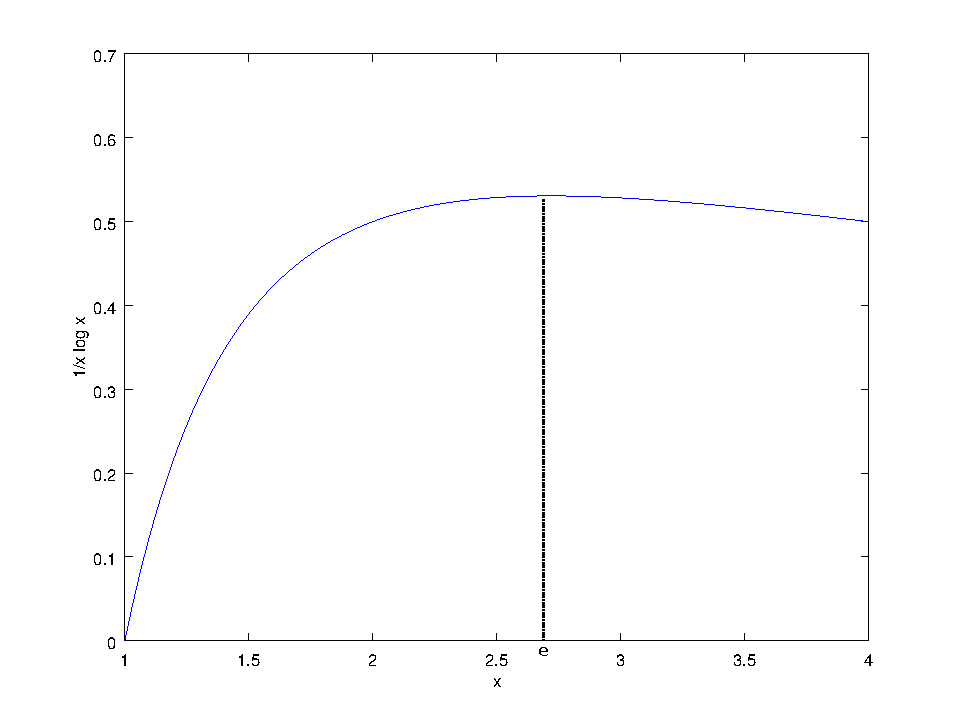
\includegraphics[width=0.6\linewidth]{images/1xlogx.pdf}

  \proofbreak
  Então, para $n \rightarrow \infty$, teremos 
  \begin{eqnarray}
  \frac{c}{n} \log \frac{n}{c} &\leq& \frac{\frac{n}{\log n} (1 + o(1))}{n} \log \frac{n}{\frac{n}{\log n} (1 + o(1))} \nonumber \\
	&=& \log \left( \log \frac{n}{1 + o(1)} \right) \frac{1 + o(1)}{\log n} \nonumber \\
	&\leq& O \left( \frac{\log \log n}{\log n} \right) \rightarrow 0 .
  \end{eqnarray}
  Concluímos assim que $\frac{c}{n} H(U,V) \rightarrow 0$ quando $n \rightarrow \infty$.

  \proofbreak
  Assim
  \begin{equation}
  \frac{c(n) \log c(n)}{n} \leq - \frac{1}{n} \log Q_k(x_{1:n}|s_1) + \epsilon_k(n)
  \end{equation}
  onde $\epsilon_k(n) \rightarrow 0$ quando $n \rightarrow \infty$.

  Desta forma,
  \begin{eqnarray}
   \limsup_{n \rightarrow \infty} \frac{c(n) \log c(n)}{n} &\leq& \lim_{n \rightarrow \infty} - \frac{1}{n} \log Q_k(x_{1:n}|X_{-(k-1):0}) \nonumber \\
	&=& H(X_0 | X_{-1}, X_{0}, \ldots, X_k)  \text{ \scriptsize para processo estacionário ergódico} \nonumber \\
	&\rightarrow& H(\mathcal{X}) \text{ quando } k \rightarrow \infty .
  \end{eqnarray}

  \end{proof}
\end{frame}



\begin{frame}[allowframebreaks]
  \frametitle{Comprimentos}

  \begin{theorem}
  Seja $X_i$ um processo estocástico estacionário de comprimento infinito.
  Seja $l(x_{1:n})$ os comprimentos das palavras LZ para $n$ símbolos. Então
	\begin{equation}
	\limsup_{n \rightarrow \infty} \frac{1}{n} l(x_{1:n}) \leq H(\mathcal{X}) 
	\end{equation}
  \end{theorem} 

  \framebreak
  \begin{proof}
  \begin{itemize}
  \item Sabemos que $l(x_{1:n}) = c(n) ( \log(c(n)) + 1 )$, onde $c(n)$
	é o número de frases da análise LZ (distintas).
  \item Pelo lemma anterior temos que
	\begin{equation}
        \limsup_{n \rightarrow \infty} \frac{c(n)}{n} = \limsup_{n \rightarrow \infty} \frac{ 1 + o(1)}{\log n} = 0 
        \end{equation}

  \item Portanto
	\begin{eqnarray}
	\limsup_{n \rightarrow \infty} \frac{ l(x_{1:n}) }{n} &=& 
		\limsup_{n \rightarrow \infty} \left( \underbrace{\frac{c(n) \log c(n)}{n}}_{\rightarrow H(\mathcal{X})} + 
		\underbrace{\frac{c(n)}{n}}_{\rightarrow 0} \right) \leq H(\mathcal{X}) .
	\end{eqnarray}

  \end{itemize}
  \end{proof}

  \begin{itemize}
  \item Em outras palavras, um algoritmo procedural (LZ), quando lida com um processo
	estocástico estacionário ergódico governado por uma dada distribuição, 
	sem a necessidade de conhecer a distribuição e apenas seguindo os passos do
	algoritmo, irá convergir pra a taxa de entropia do processo estocástico, no limite.
  \end{itemize}
\end{frame}

